\documentclass[conference]{IEEEtran}
\IEEEoverridecommandlockouts
% The preceding line is only needed to identify funding in the first footnote. If that is unneeded, please comment it out.
\usepackage{cite}
\usepackage{amsmath,amssymb,amsfonts}
\usepackage{algorithmic}
\usepackage[spanish]{babel}
\usepackage[utf8]{inputenc}
\usepackage{graphicx}
\usepackage{textcomp}
\usepackage{xcolor}
\usepackage{hyperref}
\usepackage{multirow}
\usepackage{float}
\usepackage{subcaption}
\def\BibTeX{{\rm B\kern-.05em{\sc i\kern-.025em b}\kern-.08em
    T\kern-.1667em\lower.7ex\hbox{E}\kern-.125emX}}
\begin{document}

\title{
{\large \textsc{Escuela Superior Politécnica del Litoral}\\
Administración de Sistemas Operativos - CCPG1031: Proyecto Final
}\\
Implementación de Servicio de
Telefonía IP (VoIP)\\
}

\author{\IEEEauthorblockN{\textbf{Lino Ontano}}
\IEEEauthorblockA{	\textit{Telemática}
\\Guayaquil - Ecuador \\
lontano@espol.edu.ec
}
\and
\IEEEauthorblockN{\textbf{Flavio Murillo}}
\IEEEauthorblockA{	\textit{Telemática}
\\Guayaquil - Ecuador \\
famurill@espol.edu.ec
}
\and
\IEEEauthorblockN{\textbf{Jonathan Yagual}}
\IEEEauthorblockA{	\textit{Telemática}
\\Guayaquil - Ecuador \\
jonosyag@espol.edu.ec
}
}


\maketitle

\begin{abstract}
	Este proyecto permitirá aprender las bases necesarias para la elaboración de una central telefónica (PBX) con software gratuito.
\end{abstract}

\begin{IEEEkeywords}
	PBX
\end{IEEEkeywords}
\section{Introducción}\label{sec:int}
Se ha oído hablar mucho de VoIP, con aplicaciones tan extendidas como Skype. Sin embargo,
la propuesta en este proyecto es ir algo más allá y poner en funcionamiento nuestra propia
centralita telefónica PBX basada en VoIP. Montar una centralita telefónica propia implica
un ahorro de dinero en la compra de una centralita convencional o de VoIP, para ello se utlizará Asterisk, software distribuido bajo licencia GNU. Entre
las funcionalidades de Asterisk, es posible montar, incluso, sistemas de atención automática,contestador e integrar la telefonía IP en nuestra sitio web.
En el presente proyecto instalaremos un servidor PBX Asterisk paso a paso, configuración de su GUI FreePBX y conectaremos clientes SoftPhones para simular la funcionalidad de nuestra central telefónica.

\section{Objetivos}
\subsection{General}
\begin{itemize}
\item Montar una centralita telefónica utilizando software \textit{open source} simulando la conexión cliente servidor con otros dispositivos.
\end{itemize}

\subsection{Específicos}
\begin{itemize}
\item Configurar el servidor FreePBX en una máquina virtual que permitirá elaborar la arquitectura de nuestra centralita telefónica.
\item Crear las extensiones en el servidor para conectar clientes a nuestro servidor.
\item Realizar la conexión entre clientes utilizando \textit{Softphones} de distintas plataformas.
\end{itemize}


\section{Marco Teórico}\label{sec:ant}
\subsection{\textbf{ VoIP:}}
\textbf{Voz sobre protocolo de Internet} es un conjunto de recursos que hacen posible que la señal de voz viaje a través de Internet empleando el protocolo IP, es decir la señal se envía en forma digital, en paquetes de datos. Los protocolos de internet que se usan para enviar las señales de voz sobre la red IP se conocen como protocolos de voz sobre IP o protocolos IP.
Es muy importante diferenciar entre voz sobre IP (VoIP) y telefonía sobre IP.
\begin{itemize}
\item VoIP es el conjunto de normas, dispositivos, protocolos ―en definitiva, la tecnología― que permite transmitir voz sobre el protocolo IP.
\item La telefonía sobre IP es el servicio telefónico disponible al público, por tanto con numeración E.164, realizado con tecnología de VoIP.\footnote{Tampoco se debe confundir «telefonía sobre IP» con ToIP (text over IP: ‘texto sobre IP’).}
\end{itemize}
\begin{figure}[h]
	\centerline{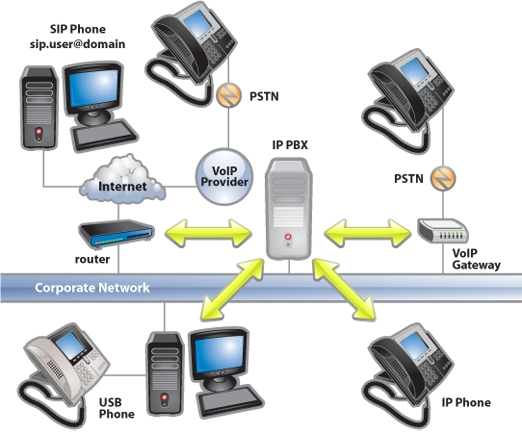
\includegraphics[width=0.3\textwidth]{img/voip01.jpg}}
	\caption{Componentes de una central telefónica VoIP}
	\label{fig:ant00}
\end{figure}
Los elementos que forman parte de un servicio VoIP son los siguientes:
\begin{itemize}
\item \textbf{Cliente}: es el que establece las llamadas de voz, se recibe a través del micrófono del usuario (entrada de información) se codifica, se empaqueta y, de la misma forma, esta información se decodifica y reproduce (salida de la información).\\
Un cliente puede ser un usuario de Skype o un usuario de alguna empresa que venda sus servicios de telefonía sobre IP o teléfonos IP o \textit{Softphones} que es un software que permite realizar llamadas a través de una computadora conectada a internet.

\item \textbf{Servidores}: son los que se encargan de manejar operaciones de base de datos, realizado en un tiempo real como en uno fuera de él. Entre estas operaciones se tienen la contabilidad, la recolección, el enrutamiento, la administración y control del servicio, el registro de los usuarios.\\
Usualmente en los servidores se instala software denominados Switches o IP-PBX (conmutadores IP), ejemplos de switches pueden ser "Voipswitch", "Mera", "Nextone", entre otros, y de IP-PBX pueden ser los de Alcatel-Lucent, Cisco o Avaya en marcas comerciales y Asterisk de código abierto. Para el presente proyecto se utilizará Asterisk.
\item \textbf{Gateways}: brindan un puente de comunicación entre todos los usuarios, su función principal es la de proveer interfaces con la telefonía tradicional adecuada, la cual funcionará como una plataforma para los usuarios (clientes) virtuales. Los gateways se utilizan para terminar la llamada, es decir: el cliente origina la llamada y el gateway termina la llamada, eso es cuando un cliente llama a un teléfono fijo o celular, debe existir la parte que hace posible que esa llamada que viene por internet logre conectarse con un cliente de una empresa telefónica fija o celular.
\end{itemize}
\subsection{\textbf{ IP-PBX:}}
Un conmutador IP o PBX por sus siglas en inglés de “Private Branch eXchange”, es la evolución de los viejos conmutadores basados en TDM; una red telefónica privada que es utilizada dentro de una empresa. En la actualidad, la era de las Comunicaciones Unificadas, los conmutadores IP ya no son simples plataformas de voz como lo eran antes. Un línea muy delgada separa las Comunicaciones Unificadas y la Telefonía IP.\\
Un Conmutador IP o PBX IP conecta las extensiones internas dentro de una empresa y al mismo tiempo las conecta con la red pública conmutada, conocida también como PSTN (Public Switched Telephone Network), Proveedores VoIP y Troncales SIP, como se observa en la figura \ref{fig:ant00}.
\subsection{\textbf{ Asterisk:}}
\begin{figure}[h]
	\centerline{
\includegraphics[width=0.2\textwidth]{img/asterisk01.png}}
	\caption{Logo de Asterisk}
	\label{fig:ant02}
\end{figure}
\textit{Asterisk} es un programa de software libre (bajo licencia GPL) que proporciona funcionalidades de una central telefónica (PBX). Como cualquier PBX, se puede conectar un número determinado de teléfonos para hacer llamadas entre sí dentro de una misma organización e incluso acceder a comunicaciones fuera de la misma a la PSTN o conectando a un proveedor de VoIP o bien a una RDSI tanto básicos como primarios. Originalmente desarrollado para el sistema operativo GNU/Linux, \textit{Asterisk} actualmente también se distribuye en versiones para los sistemas operativos BSD, Mac OS X, Solaris y Microsoft Windows, aunque la plataforma nativa (GNU/Linux) es la que cuenta con mejor soporte de todas.\\
\begin{figure}[h]
	\centerline{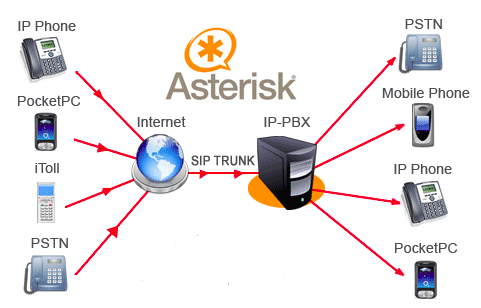
\includegraphics[width=0.5\textwidth]{img/asteriksvoip00.png}}
	\caption{Arquitectura de una red con \textit{Asterisk}}
	\label{fig:ant03}
\end{figure}
\textit{Asterisk} incluye muchas características que anteriormente sólo estaban disponibles en costosos sistemas propietarios PBX, como buzón de voz, conferencias, IVR, distribución automática de llamadas, y otras muchas. Los usuarios pueden crear nuevas funcionalidades escribiendo un dialplan en el lenguaje de script de \textit{Asterisk} o añadiendo módulos escritos en lenguaje C o en cualquier otro lenguaje de programación soportado en GNU/Linux.\\
Uno de los puntos fuertes del software \textit{Asterisk} es que permite la unificación de tecnologías: VoIP, GSM y PSTN.\\
\textit{Asterisk} se empieza a adoptar en algunos entornos corporativos como una gran solución de bajo coste junto con SER (Sip Express Router).


\subsection{\textbf{ FreePBX:}}
\textit{FreePBX} es una GUI (interfaz gráfica de usuario) de código abierto basado en web que controla y dirige \textit{Asterisk}. \textit{FreePBX} está licenciado bajo la GNU General Public License y es un componente del FreePBX Distro (una distribución de GNU/Linux, basada en CentOS con el sistema PBX pre-instalado).
\begin{figure}[h]
	\centerline{
\includegraphics[width=0.25\textwidth]{img/freepbx01.png}}
	\caption{Logo de FreePBX Distro}
	\label{fig:ant04}
\end{figure}


\section{Metodología}\label{sec:met}
\begin{figure}[h]
	\centerline{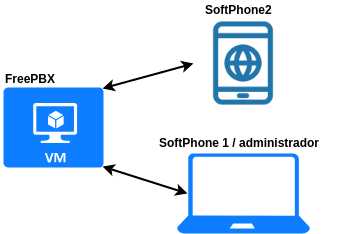
\includegraphics[width=0.3\textwidth]{img/diagrama01.png}}
	\caption{Diagrama a implementar con FreePBX como servidor y dos clientes}
	\label{fig:ddc01}
\end{figure}

Para el desarrollo de nuestro proyecto, lo haremos de manera local por medio de una máquina virtual que hará de servidor y en cual se conectará dos clientes, un dispositivo móvil y una laptop, donde la laptop hará de cliente y de administrador ya que tendrá acceso a la interfaz gráfica de FreePBX para su administración. En los clientes los dispositivos harán de \textit{softphones}, con diferentes software para cada uno en el cual no entraremos en detalle dado que nos interesa la administración del servidor de nuestra central telefónica que le brindará servicio a esos dos clientes.
Para la configuración de nuestra centralita telefónica, lo hemos divido en dos partes, la configuración de nuestro servidor y la configuración en los \textit{softphones} de cada cliente, que en este caso es de distinto tipo de dispositivo.

\subsection{Configuración Servidor}
\begin{figure}[h]
    \begin{subfigure}[h]{0.5\textwidth}
       \centerline{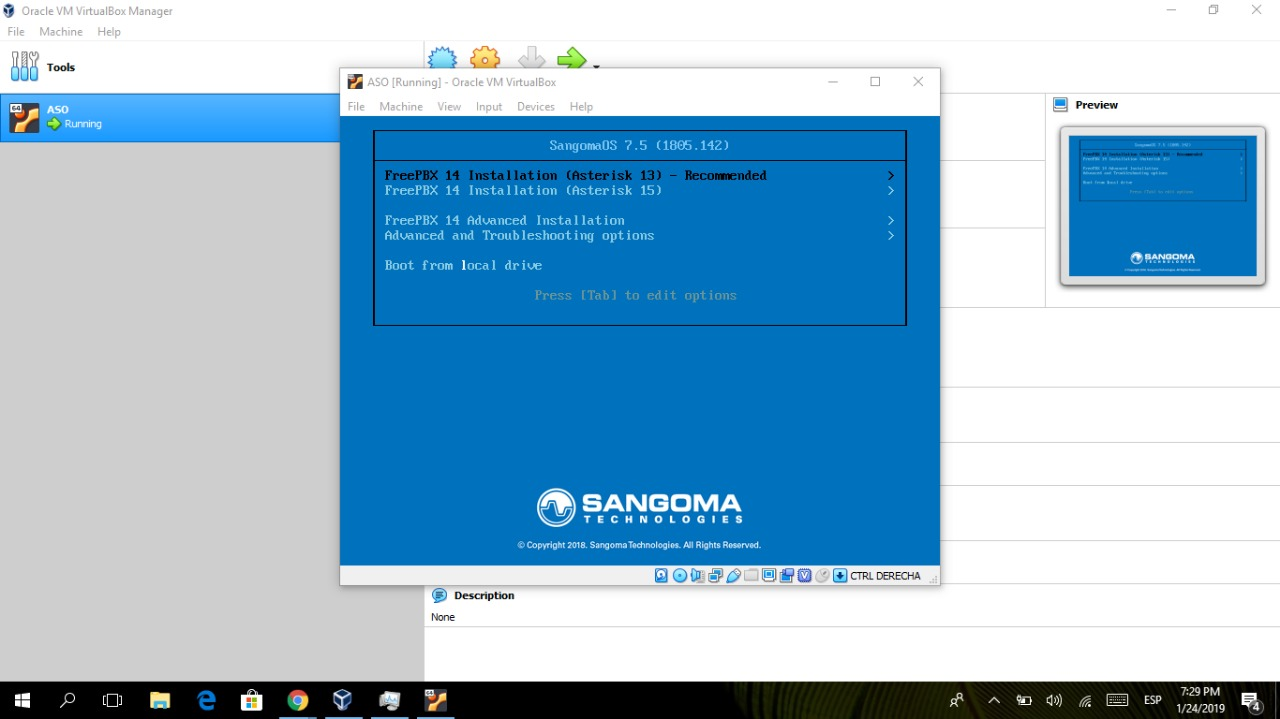
\includegraphics[width=0.7\textwidth]{img/1.jpeg}}
        \caption{Selección de versión de FreePBX}

    \end{subfigure}
    ~ %add desired spacing between images, e. g. ~, \quad, \qquad, \hfill etc.
     \begin{subfigure}[h]{0.5\textwidth}
        \centerline{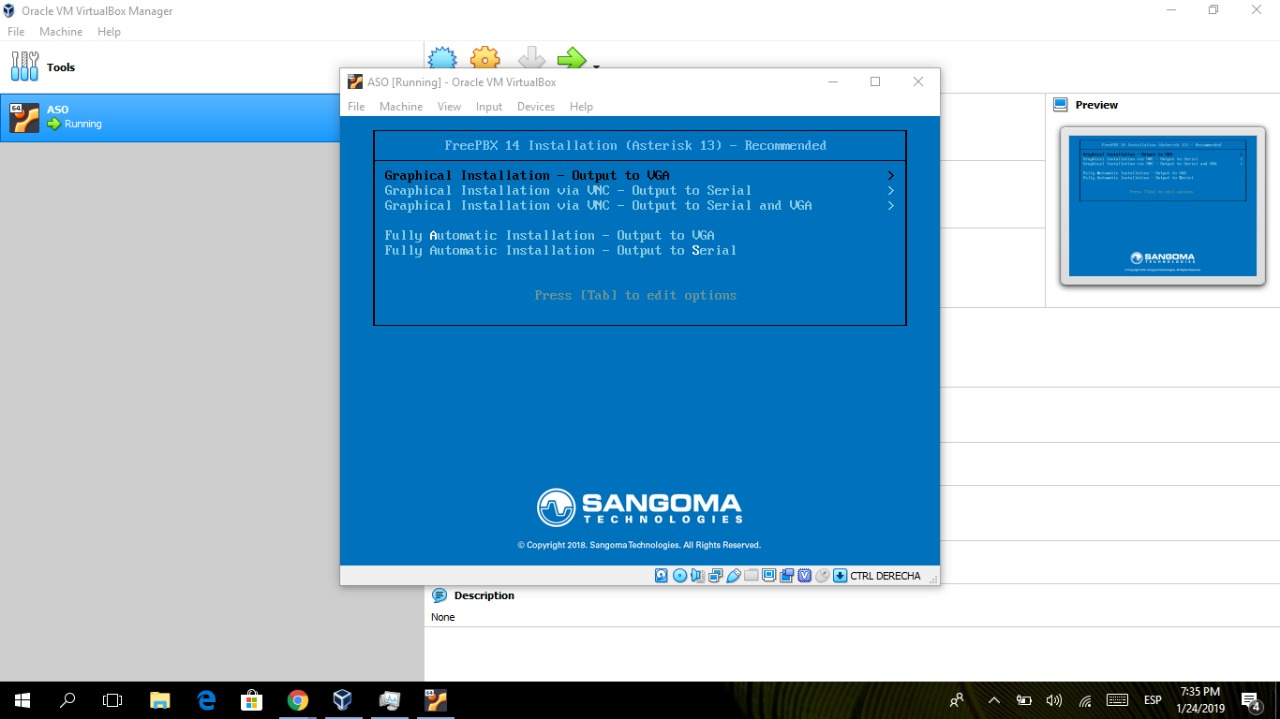
\includegraphics[width=0.7\textwidth]{img/2.jpeg}}
        \caption{Instalación de la parte gráfica de FreePBX}

    \end{subfigure}
    \caption{\textit{Instalación del servidor FreePBX.}}
\label{fig:mets0}
\end{figure}
En primer lugar se requiere el \texttt{.iso} del servidor FreePBX que utilizaremos. Se lo puede descargar desde el sitio de \href{https://www.freepbx.org/downloads/freepbx-distro/}{{\textbf{FreePBX}}}. Una vez descargado y montado en nuestra máquina virtual procedemos con la instalación del servidor. Seguimos los pasos como se muestra en la figura \ref{fig:mets0}.\\

Una vez seleccionado las componentes a instalar, empezará la instalación donde pedirá la creación de un usuario y contraseña. Una vez terminado de instalar, arrancará el servidor indicando la configuración de red actual que posee para acceder de manera remota por medio de su interfaz gráfica.\\
Ya en este punto, se puede acceder al servidor y configurar las extensiones para los clientes. En una centralita telefónica genera extensiones a los dispositivos clientes para que ellos, por medio de una autenticación de usuario, acceda a esa extensión del servidor y pueda comunicarse con cualquier extensión de la central. Esto lo realizamos accediendo a la interfaz gráfica desde cualquier navegador conectado en la misma red del servidor y poniendo la dirección ip del servidor. Para la configuración del servidor pedirá las credenciales que se crearon en la parte de la instalación previa.
\begin{figure}
	\centerline{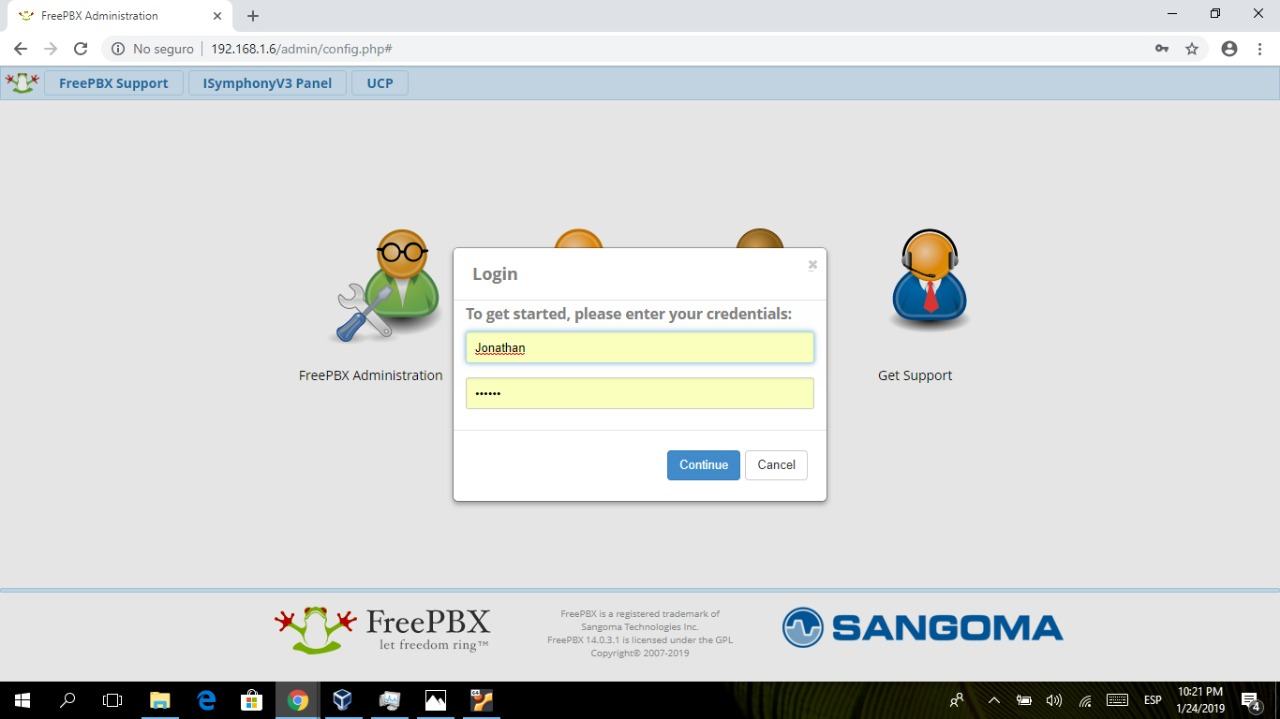
\includegraphics[width=0.45\textwidth]{img/8.jpeg}}
	\caption{\textit{Acceso al servidor FreePBX.}}
	\label{fig:mets2}
\end{figure}
Agregamos las extensiones para dos dispositivos, la extensión 101 y 102. Para agregar una extensión utilizaremos el protocolo SIP para comunicación. Y añadiremos los datos para que el cliente pueda acceder a esa extensión.
\begin{figure}
	\centerline{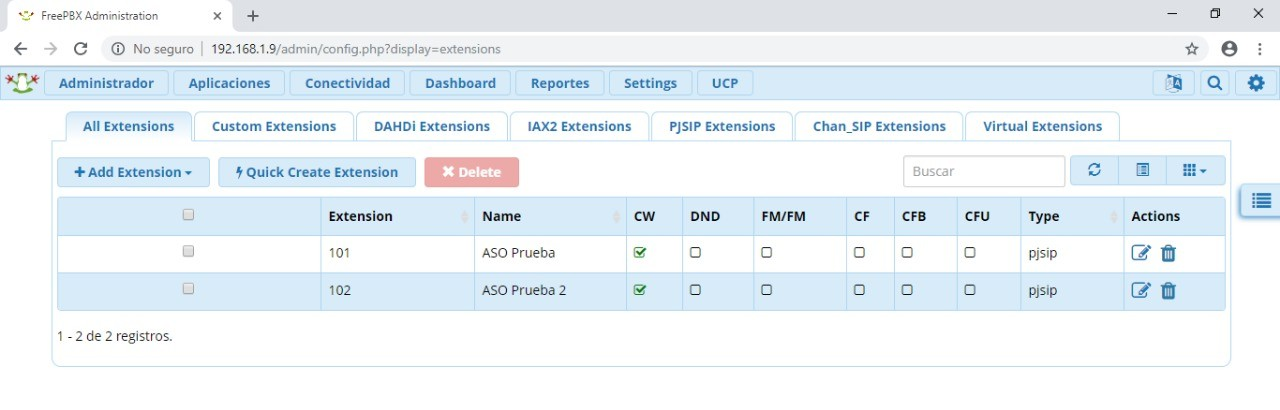
\includegraphics[width=0.5\textwidth]{img/mets04.jpeg}}
	\caption{\textit{Directorio de extensiones.}}
	\label{fig:mets4}
\end{figure}
Una vez creado nuestro directorio de extensiones, tendremos que configurar nuestro \textit{softphones} para que accedan a ello.

\subsection{Configuración Cliente}
\begin{figure}[h]
    \begin{subfigure}[h]{0.35\textwidth}
       \centerline{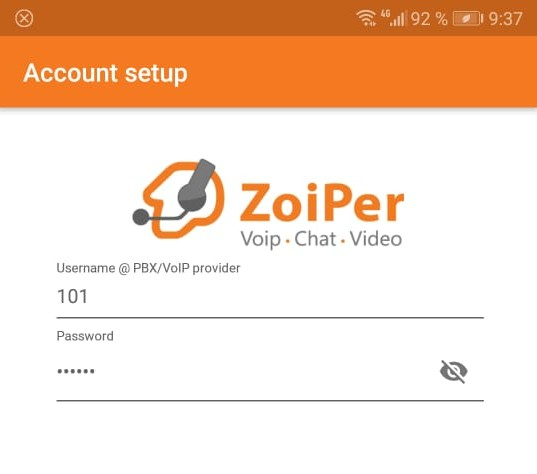
\includegraphics[width=0.7\textwidth]{img/metc01.jpeg}}
        \caption{Inicio de sesión desde dispositivo móvil}

    \end{subfigure}
    ~ %add desired spacing between images, e. g. ~, \quad, \qquad, \hfill etc.
     \begin{subfigure}[h]{0.35\textwidth}
        \centerline{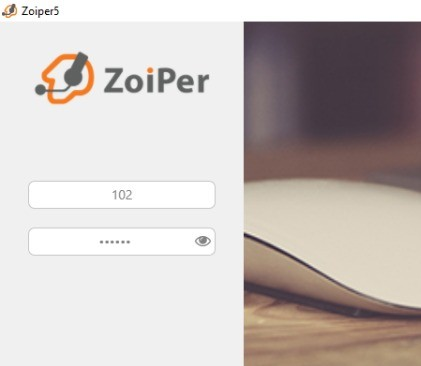
\includegraphics[width=0.7\textwidth]{img/metc02.jpeg}}
        \caption{Inicio de sesión desde la aplicación de escritorio.}

    \end{subfigure}
    \caption{\textit{Configuración de Zoiper.}}
\label{fig:metc0}
\end{figure}
El \textit{softphone} a utilizar para elaborar la comunicación VoIP es \href{https://www.zoiper.com/}{{\textbf{Zoiper}}}, que es gratuito y multiplataforma. Utilizaremos en un dispositivo móvil y en una laptop. Lo que se realiza es acceder al servidor FreePBX con la extensión como username y la contraseña de la misma extensión configurada en el servidor; de esta manera, en el dispositivo se habilita dicha extensión para la comunicación. Toda esta configuración se observa en la figura \ref{fig:metc0}.\\ Ya realizado esto, se puede realizar llamadas entre extensiones desde cualquier \textit{softphone}. Se puede observar, además, que los dispositivos están configurados con el servidor FreePBX.
\begin{figure}[h]
    \begin{subfigure}[h]{0.35\textwidth}
       \centerline{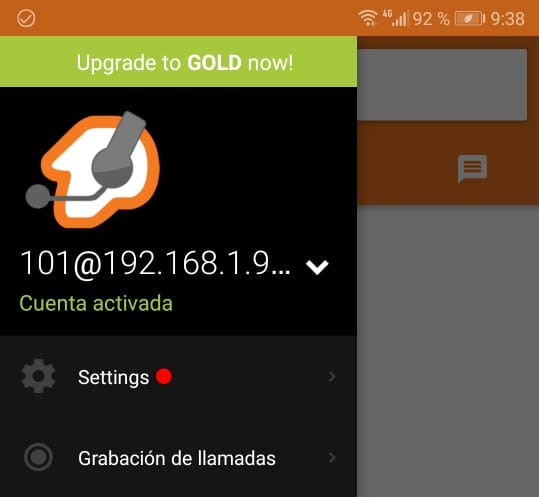
\includegraphics[width=0.7\textwidth]{img/metc03.jpeg}}
        \caption{Zoiper configurado en dispositivo móvil}

    \end{subfigure}
    ~ %add desired spacing between images, e. g. ~, \quad, \qquad, \hfill etc.
     \begin{subfigure}[h]{0.35\textwidth}
        \centerline{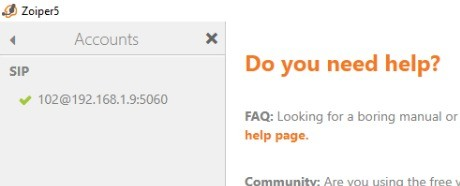
\includegraphics[width=0.7\textwidth]{img/metc04.jpeg}}
        \caption{Zoiper configurado en la aplicación de escritorio.}

    \end{subfigure}
    \caption{\textit{Dispositivos con Zoiper.}}
\label{fig:metc0}
\end{figure}


\section{Resultados}
\begin{figure}[H]
    \begin{subfigure}[h]{0.5\textwidth}
       \centerline{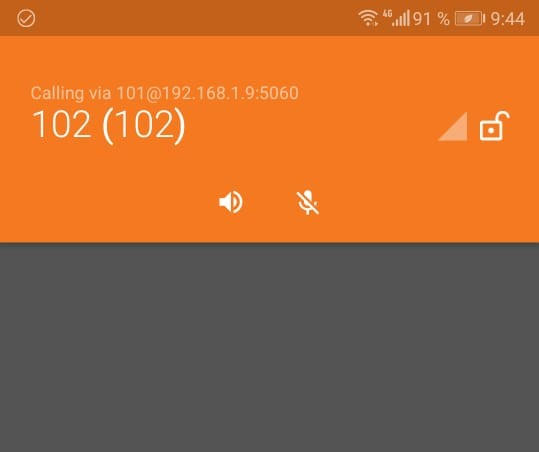
\includegraphics[width=0.7\textwidth]{img/metc05.jpeg}}
        \caption{Llamada desde la extensión 101 a la extensión 102.}

    \end{subfigure}
    ~ %add desired spacing between images, e. g. ~, \quad, \qquad, \hfill etc.
     \begin{subfigure}[h]{0.5\textwidth}
        \centerline{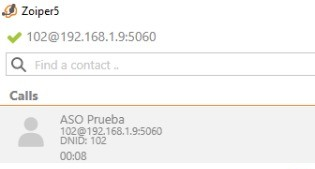
\includegraphics[width=0.7\textwidth]{img/metc06.jpeg}}
        \caption{Llamada recibida desde la extensión 101.}

    \end{subfigure}
    \caption{\textit{Llamadas entre extensiones.}}
\label{fig:metc3}
\end{figure}

\section{Análisis de Resultados}
La configuración del servidor y de los clientes fueron realizados con éxito, y se logró la comunicación sobre VoIP con software \textit{open source}. Hay que aclarar que la seguridad depende en su parte en el \textit{softphone}, por ejemplo en nuestro caso Zoiper encripta las comunicaciones lo que presenta mayor seguridad en nuestra centralita. A parte de las autenticaciones que se realizan desde el servidor con los clientes que acceden al directorio de extensiones. La demostración que realizamos es una llamada desde la extensión 101 hacia la extensión 102, y se observa en la figura \ref{fig:metc3} como la extensión recibe la llamada desde la extensión 101.


\section{Conclusiones}
\begin{itemize}
	\item La transmisión de voz sobre IP puede facilitar el proceso de incrementar las líneas telefónicas en la empresa sin la necesidad de líneas físicas adicionales.
	\item El uso de este tipo de software incluye funcionalidades que normalmente son facturadas con cargo extra por las compañías de teléfonos, tales como transferencia de llamadas, identificación de la persona que llama o remarcado automático, son fáciles de implementar con la tecnología de voz sobre IP.
  \item FreePBX surge como un panel web de código abierto para Asterisk, facilitando la configuración de funciones de Asterisk de forma gráfica sin necesidad de requerir conocimientos elevados de programación.
\end{itemize}

\section{Recomendaciones}
\begin{itemize}
	\item Prestar mucha atención a las credenciales de los usuarios dado que son necesarias para la configuración en otros dispositivos, el ingreso incorrecto de las mismas puede ocasionar caídas en el servidor.
	\item Asegurarse de que las extensiones creadas usen los protocolos disponibles en los softphones para evitar conflictos en el registro de cuentas.
  \item Verificar que los dispositivos a registrar se encuentren todos dentro de la misma red local.
\end{itemize}


\begin{thebibliography}{00}
\bibitem{b1}  Google Talkabout, ``XMPP Federation'' , 2006.
\bibitem{b2} Shead, Sam, ``Android SIP Client", ZDNet, Octubre 2012.
\bibitem{b3} Michael Dosch, Steve Church, ``VoIP in the Broadcast Studio''  Axia Audio, 2011.
\bibitem{b4} A.H. Muhammad Amin, ``VoIP performance measurement using QoS parameters,''  2016.
\bibitem{b5} Madsen, Leif, Jim Van Meggelen; ``Asterisk: The Definitive Guide, 4th Edition", O'Reily Media, 2013.
\end{thebibliography}

\end{document}
